\chapter{Pion Cloud Effect}
\label{chap:pion}
There are, however, also severe limitations to the 
rainbow-ladder scheme. Consequently, much work has been 
invested in the past years on its extension towards more 
advanced approximations of the quark-gluon interaction. 
On the one hand, this may be accomplished directly by devising
improved \textit{ans\"atze} for the dressing functions of the 
quark-gluon vertex 
\cite{Fischer:2005en,Chang:2009zb,Chang:2010hb,Heupel:2014ina}.
On the other hand, it is promising to work with diagrammatic
approximations to the vertex DSE. While most studies so far concentrated 
on ($1/N_c$-subleading) Abelian contributions to the vertex (see e.g. 
\cite{Bender:1996bb,Watson:2004kd,Watson:2004jq,Bhagwat:2004hn,Matevosyan:2006bk}),
the impact of the $1/N_c$-leading, non-Abelian diagram on light meson
masses has been investigated in \cite{Fischer:2009jm}. In addition,
important unquenching effects in the quark-gluon interaction may 
be approximated by the inclusion of hadronic degrees 
of freedom \cite{Fischer:2007ze,Fischer:2008sp,Fischer:2008wy}. 
This is possible, since the vertex DSE can be decomposed on a diagrammatic
level into terms that are already present in the quenched theory and those 
involving explicit quark-loops. The latter ones can be expressed involving  
hadronic degrees of freedom. To leading order in the hadron masses, pion 
exchange between quarks is dominating these contributions. These pions are 
not elementary fields. Consequently, their wave functions need to be determined 
from their Bethe-Salpeter equation. \\

Having explicit hadronic degrees of freedom in the system may also be very 
beneficial for phenomenological applications of the approach. Pion cloud effects 
are expected to play an important role in the low momentum behavior of 
form factors and hadronic decay processes of baryons
\cite{Thomas:1981vc,Miller:2002ig,Ramalho:2008dp,Cloet:2012cy,Eichmann:2011vu,
Eichmann:2011aa,Sanchis-Alepuz:2013iia}. Within the covariant BSE-approach, 
the influence of pion back-coupling effects in the mass and decay 
constants of the pion itself and other light mesons has been studied in \cite{Fischer:2008wy}. 
In the present work, we take this framework one step further and extend it 
to the covariant three-body calculations of nucleon and delta masses 
\cite{Eichmann:2009qa,Eichmann:2009en,SanchisAlepuz:2011jn}. 

\section{Mesons}
From technical point of view the meson \BSE with pion cloud effect, provided by the changes to the two-quark scattering kernel $K$
given in Chapter \ref{chap:BSE}, represents the similar eigenvalue value problem. Therefore we can apply the same numerical machinery 
in order to obtain mass spectra and \BS vertex functions. Recall, the total scatterintg kernel takes the following form:
\beqa
	K(p,k;P) = K^{gluon}(p,k;P) + K^{pion}(p,k;P)\;
\eeqa
However, since we include the unquenching effects in to the total kernel $K$, the gluon rainbow-ladder part $K^{gluon}$, 
\begin{table*}[!h]
 \begin{center}
 \small
\renewcommand{\arraystretch}{1.2}
  \begin{tabular}[h]{c||c|c|c|c|}
\hline
\hline
  [MeV]  & RL1   & RL2      & RL2 + $\pi$ & Exp. \\ \hline\hline
 $m_\pi$ & 138	 & 144 & 138  & 138\\ 
 $f_\pi$ & 93	 & 98 & 93    & 93\\ 
 $\langle q\bar{q}\rangle^{1/3}_{\mu=19 \,\text{GeV}}$
        & 281  & 300 & 280  &   \\ \hline\hline
 $m_\rho$ & 757  & 855 & 766  & 776 \\
 $m_\sigma$& 643 & 724 & 610 & 400-1200 \\
 $m_{a_1}$ & 969 & 1115 & 1052 & 1260\\
 $m_{b_1}$ & 852 & 1007 & 941 & 1235\\
 $m_{a_2}$ & 1154 & 1389 & 1302 & 1320\\  
 $m_{\pi_2}$ & 1202 & 1456 & 1373 & 1670\\  
 $m_{\rho_3}$& 1528 & 1791 & 1673 & 1690\\  
 \hline\hline
\end{tabular}
\caption{Meson mass spectrum, decay constant and the chiral condensate for single gluon exchange (RL1), including the pion 
cloud corrections corrections (RL2 + $\pi$) and with the pion cloud switched off, but the effective interaction (RL2) unchanged, compared with experimental values.\label{tab:masses_mesons}}
 \end{center}
\end{table*}
\begin{figure}[!h]
\begin{center}
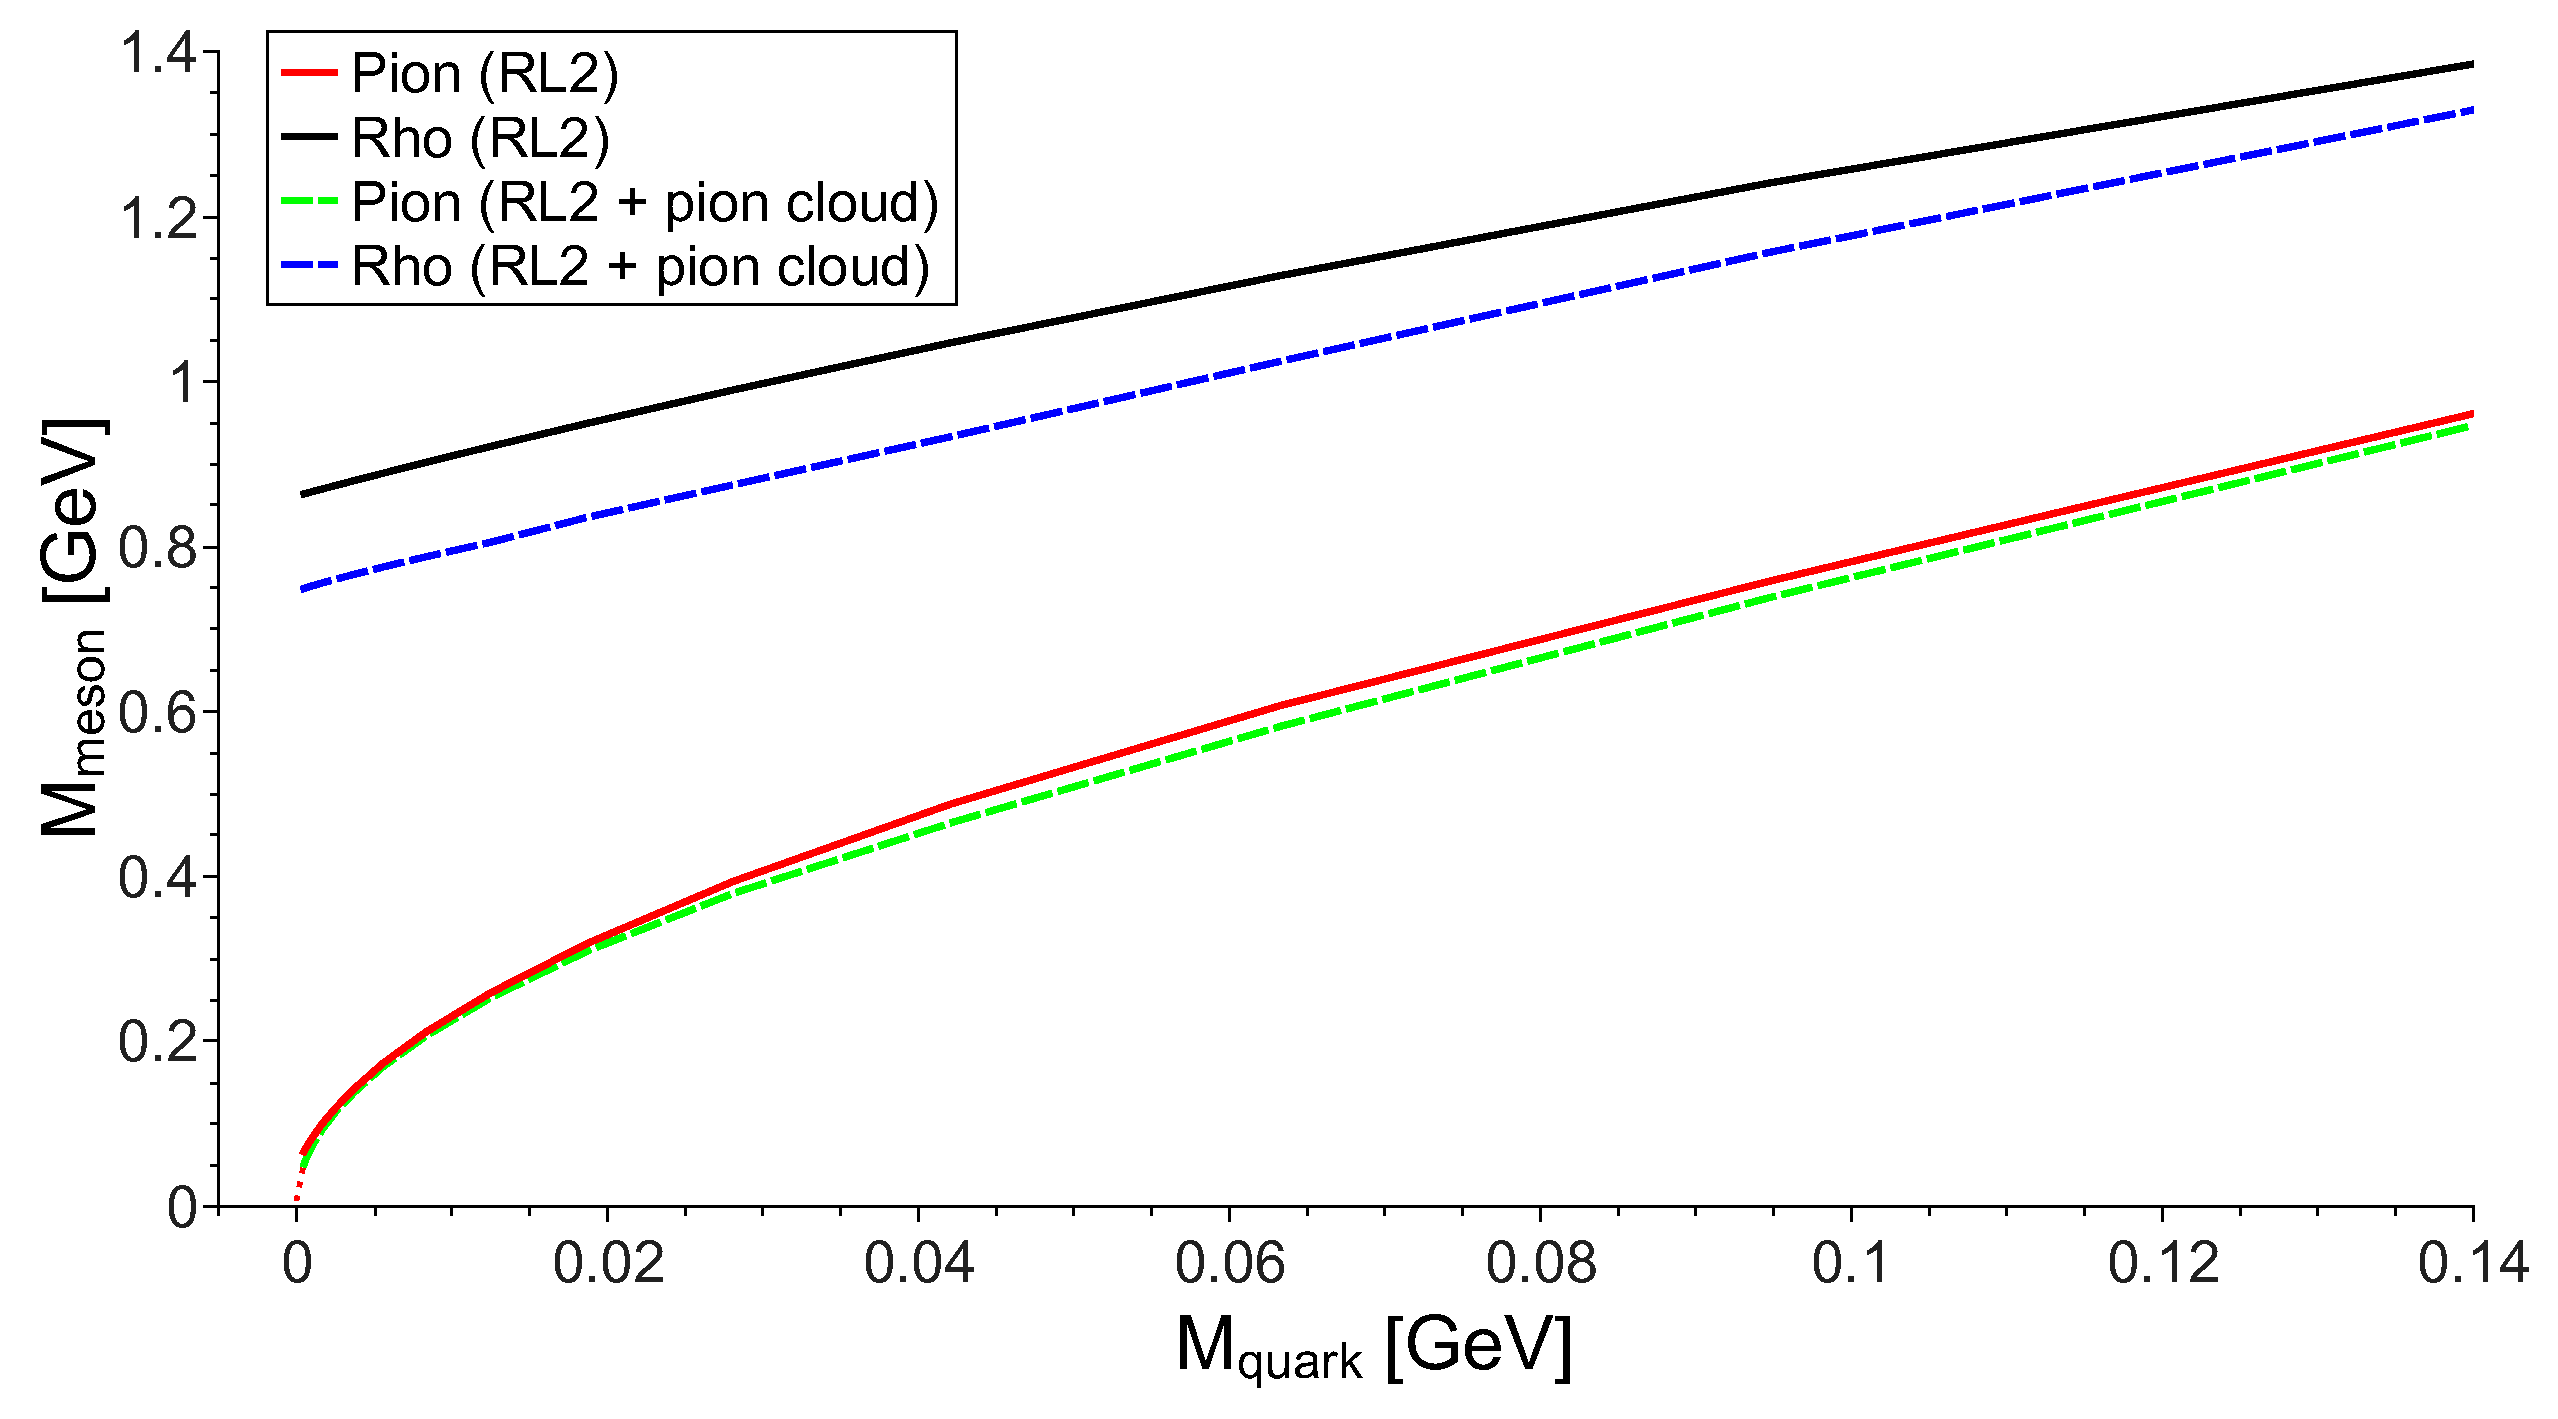
\includegraphics[width=0.99\textwidth]{figures/GMOR_Pi} 
\caption{\footnotesize Masses of pion and rho as functions of quark mass. The Gell-Mann-Oakes-Renner relation is indicated. }\label{fig:GMOR}
\end{center}
\end{figure}
representing effective single gluon exchange must change its parameters $\Lambda$ and $\eta$ in order to incorporate the withdraw of the hadronic contribution into the explicit part $ K^{pion}$. 
The parameters are $\Lambda=0.84$ and $\eta=1.8$ as given in Table. \ref{tab:RL_params}. It is also interesting to perform the calculations with and without the pion cloud effect switched on to draw some insights on size on unquenching effects. The results on meson masses, decay constant and the chiral condensate are given on Table. \ref{tab:masses_mesons}. The general trend is that inclusion of the pion cloud effect provides lighter spectrum in comparison to RL2 by generating a downwards shift in average 70-130 MeV.  \\

The complete interaction kernel consisting of
the rainbow-ladder gluonic diagram and the pion exchange diagram does
satisfy the axial-vector Ward-Takahashi identity. This can be demonstrated 
analytically \cite{Fischer:2007ze,Fischer:2008wy} and holds even with the
approximation of the exchanged pion's Bethe-Salpeter amplitude. As a result,
using this interaction kernel one obtains a pseudoscalar Goldstone boson
in the chiral limit and the holding Gell-Mann-Oakes-Renner relation \cite{Fischer:2007ze,Fischer:2008wy} as it shown on Fig. \ref{fig:GMOR}. 
Since this truncation scheme does not contain the t-channel two-pion exchange diagram for the $\rho$ to decay into pions, we do not observe
the specific behaviour of the rho mass as the pion mass reaches threshold $m_\pi>m_\rho/2$, due to the opening of a decay channel \cite{Allton:2005fb}. The impact on baryon masses will be considered in the next chapter. \\

%\subsection*{Photon-quark vertex}
\section{Baryons}
\label{sec:results}

\begin{table*}[t]
 \begin{center}
 \small
\renewcommand{\arraystretch}{1.2}
  \begin{tabular}[h]{|c||c|c|c|c|}\hline
  [GeV]     &  RL1     & RL2      & RL2 + $\pi$ & Exp. \\ \hline\hline
 $m_\pi$  	& 0.138 (1)& 0.144 (1)& 0.138 (1)   & 0.140\\ \hline
 $f_\pi$  	& 0.093 (1)& 0.098 (1)& 0.093 (1)   & 0.093\\ \hline
 $\langle q\bar{q}\rangle^{1/3}_{\mu=19 \,\text{GeV}}$
          	& 0.281 (2)& 0.300 (3)& 0.280 (3)    &      \\ \hline\hline
 $m_N$      & 0.94 (1) & 1.01 (3) & 0.86 (1)    & 0.94 \\ \hline
 $m_\Delta$ & 1.23 (1) & 1.36 (1) & 1.30 (3)    & 1.23 \\ \hline
\end{tabular}
\caption{Nucleon and Delta masses as well as pion mass, decay constant and the chiral condensate 
using the rainbow-ladder truncation only (RL1),
rainbow-ladder with the refitted effective interaction (RL2) and including the pion 
cloud corrections corrections (RL2 + $\pi$). 
We give the central value of the bands corresponding to a variation of 
$\eta$ between $1.6 \le \eta \le 2.0$ with the halfwidth of the bands added in brackets. 
We compare also with experimental values.\label{tab:masses}}
 \end{center}
\end{table*}

\begin{figure*}[t]
\begin{center}
  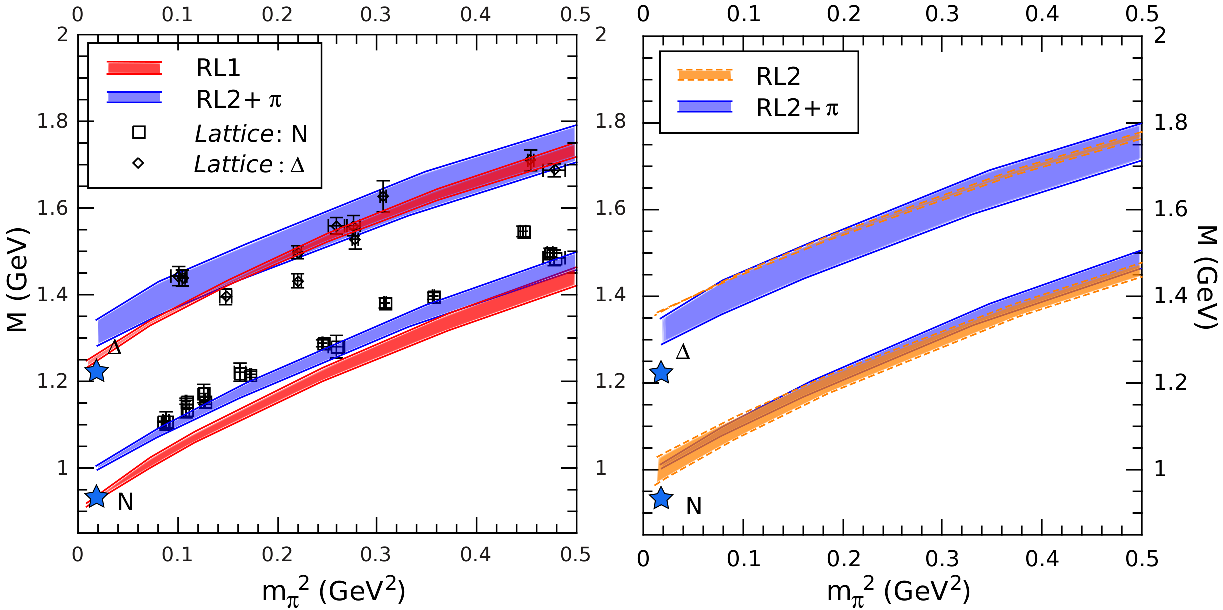
\includegraphics[width=0.99\textwidth]{figures/eta-bands}
 \end{center}
 \caption{Evolution of the nucleon and delta mass with respect to the pion mass squared. \textit{Left panel}: We plot the results for pure RL1 and for RL2 with pion exchange. We also compare with a selection of (unquenched) 
lattice data \cite{Alexandrou:2006ru}-\cite{Gattringer:2008vj}. \textit{Right panel}: We compare the results for RL2 only and RL2 with pion exchange. Stars denote the physical nucleon and delta mass.
The shaded bands correspond to a variation of the interaction parameter $\eta$ between
$1.6 \le \eta \le 2.0$, with $\eta=1.6$ corresponding to the upper limit of the bands.}\label{fig:mass_panel}
\end{figure*}

To proceed with the calculations we must fix the two parameters $\Lambda$ 
and $\eta$ of the interaction as well as the 
current-quark masses. This is conveniently done by using the 
experimental values for the pion decay constant $f_\pi$ and the pion mass $m_\pi$
as benchmark. The pion decay constant is largely insensitive to the 
current quark mass, which is consequently fixed by the physical pion mass.
On the other hand, the parameter $\Lambda$ corresponds to an interaction 
scale, and is therefore in one-to-one relation with $f_\pi$. Furthermore,
it has been noted that the pion decay constant can only be reproduced by 
a range of values of $\eta$ between $1.6$ and $2.0$ (see, e.g. 
\cite{Eichmann:2011vu,Krassnigg:2009zh}). 
For the pure RL interaction $\widetilde{K}^{RL}$ the resulting values for $\Lambda$ and the quark mass
are $\Lambda=0.72$~GeV and $m_{u/d}(\mu^2)=3.7$~MeV; we denote this case by RL1.
Since the pion back-reaction is not taken into account explicitly in this case,
its effects are, to some extent, encoded implicitly in the parameters (in particular the scale) 
of the interaction. This is different for the pion corrected kernel 
$\widetilde{K} = \widetilde{K}^{RL}-\widetilde{K}^{pion}$. Since pion cloud effects are 
now treated explicitly, $\widetilde{K}^{RL}$ describes 
the interactions in the bound state's quark-core only. As a result, the 
interaction range of this part of the kernel (in coordinate space) is expected to decrease, which in turn means that 
$\Lambda$ should increase \cite{Thomas:1981vc}. This is indeed what we observe: for the 
pion-corrected kernel we need $\Lambda=0.84$~GeV to reproduce $f_\pi$ with 
$\eta \in [1.6,2.0]$. The quark mass $m_{u/d}(\mu^2)=3.7$~MeV remains the same.
We use the label RL2 for the RL part of this truncation. 
The renormalisation scale in all cases is chosen to be $\mu^2= (19 \,\mbox{GeV})^2$.

\subsection*{Nucleon and Delta masses and Sigma terms}
The calculated masses of the Nucleon and the Delta, with and without the 
pion-exchange kernel, are shown in Tab.~\ref{tab:masses}. In the RL1 framework
one observes very good agreement with the experimental 
mass values. However, as shown in Ref.~\cite{Eichmann:2011vu,Eichmann:2011pv}, the 
internal structure of the nucleon as probed by electromagnetic as well as axial 
and pseudoscalar currents is not well represented at low momenta due
to missing explicit pion cloud effects. These are included (within the limits of 
our truncation) in the RL2 + $\pi$-calculation. For comparison we also display 
results for the purely gluonic rainbow-ladder part of this truncation (RL2), which
represents a quark-core calculation of the nucleon mass with stripped pion cloud.
As a result we find substantial pion cloud effects in the nucleon. Compared with 
the quark-core part (RL2) the nucleon mass is reduced by about $150$ MeV in the 
full calculation (RL2+$\pi$). Comparing RL2+$\pi$ with RL1, which both reproduce
the physical pion mass and decay constant we still find pion cloud effects of the
order of $80$ MeV. This sizable mass shift for the nucleon at the physical
point agrees qualitatively with other estimates in the literature, see e.g. 
\cite{Young:2002cj} and references therein. The corresponding mass shift in the
$\Delta$-isobar is much smaller and behaves differently. Comparing RL2 and RL2+$\pi$
we find a decrease of the $\Delta$-mass by about $60$ MeV, which is less than half
the size of the corresponding shift in the nucleon. However, when comparing with
RL1, we even find an increase in the $\Delta$-mass by about $70$ MeV. This is a
result of the different interaction scale $\Lambda$ in the two setups, which
was necessary to reproduce the physical pion decay constant correctly. As a result
we find a mass shift of different sign for the $\Delta$ than for the nucleon. \\

The evolution of the baryon masses as a function of $m_\pi^2$ (or, equivalently, 
with respect to the current-quark mass), is displayed in Fig.~\ref{fig:mass_panel},
where we also display corresponding lattice data \cite{Alexandrou:2006ru}-\cite{Gattringer:2008vj}.
In general, we observe that the inclusion of pion cloud effects increases the mass 
splitting between the nucleon and the $\Delta$ considerably. Although the size of 
this increase may be too large, its qualitative behavior is in agreement with
well-known results in the literature \cite{Thomas:1981vc}. Including the pion
cloud effects, the excellent agreement of the pure rainbow-ladder calculation RL1
with experiment is spoiled and we are left with discrepancies for the nucleon
and the $\Delta$ on the ten percent level. Whereas the mass evolution for the 
$\Delta$ is not too far away from the corresponding lattice results, the one
for the nucleon is shifted by 10-20 percent for all pion masses, although the slope 
of the evolution is more or less correct. \\

In general, however, the quantitative discrepancies of our approach with the lattice 
results indicate missing structure such as gluon self interaction effects in the
two-body kernels (see \cite{Fischer:2009jm} for a study of these in the meson 
sector), genuine three-body interactions (also mediated by gluon self interaction
contributions) and potential deficiencies in our pion exchange kernel. This
needs to be further explored in future work.  \\

An observable effect of the slope of the mass-evolution curve close to the physical
point is given by the nucleon and delta sigma terms. In our approach, these are
trivially obtained using the Feynman-Hellman theorem
\begin{equation}
 \sigma_{\pi X}=m_q\frac{\partial M_X}{\partial m_q}\,,
\end{equation}\label{eq:sigma_terms}
where $m_q$ is the current-quark mass, $M_X$ is the baryon mass and the derivative 
is taken at the physical quark mass. For the nucleon we obtain 
\begin{eqnarray}
\sigma_{\pi N} &=& 30 (3)~\mbox{MeV (RL1)}, \nonumber\\
\sigma_{\pi N} &=& 26 (3)~\mbox{MeV (RL2)}, \nonumber\\
\sigma_{\pi N} &=& 31 (3)~\mbox{MeV (RL2+$\pi$)} \label{FH1}
\end{eqnarray}
for RL1, RL2 without and RL2 with pion exchange, respectively. Likewise, we obtain 
for the delta 
\begin{eqnarray}
\sigma_{\pi \Delta} &=& 24 (2)~\mbox{MeV (RL1)}, \nonumber\\
\sigma_{\pi \Delta} &=& 23 (3)~\mbox{MeV (RL2)}, \nonumber\\
\sigma_{\pi \Delta} &=& 24 (3)~\mbox{MeV (RL2+$\pi$)}\,. \label{FH2}
\end{eqnarray}
For the pion-nucleon case both of our values using physical parameters (RL1 and RL2+$\pi$) 
are slightly below the lower bound of a range of recent lattice 
results \cite{Shanahan:2012wh,Alvarez-Ruso:2013fza,Bali:2013dpa}. From a comparison of the
quark core calculation RL2 with RL2+$\pi$ we infer that about twenty percent of the nucleon
sigma term are generated by pion cloud effects. For the $\Delta$ this fraction is considerably 
smaller and our results in general are about 30 \% lower than available model 
results \cite{Lyubovitskij:2000sf,Cavalcante:2005mb}. \\

Within certain limits, the slope can be influenced by the choice of the model
parameters as reflected in the numbers in brackets given in (\ref{FH1}) and (\ref{FH2}).
However, as mentioned above, in order to study the mass evolution of the system 
and the resulting sigma-terms in more detail, one should include 
the effects of the gluon self-interaction in the two-body and three-body 
correlations, since these may have a significant impact \cite{Fischer:2009jm}. 

\subsection*{Internal composition}\label{subsec:internal_composition}
Some insight into the internal structure of the baryon can be gained by 
studying the relative importance of the different partial-wave sectors. 
As shown in \cite{Eichmann:2009qa,Eichmann:2009en,SanchisAlepuz:2011jn}, 
Poincar\'e covariance enforces that in our framework baryons are composed, 
in principle, by s-, p- and d-wave components for spin-$\frac{1}{2}$ 
particles and s-, p-, d- and f-wave components for spin-$\frac{3}{2}$
particles. Therefore, one \textit{cannot} restrict the partial-wave 
composition in a covariant way and it is the dynamics what 
dictates the contribution of these components to a given state. Moreover, 
in the case of the nucleon, the flavor part of the Faddeev amplitude contains 
a mixed-symmetric and a mixed-antisymmetric term, as dictated by symmetry. 
Each of these is accompanied by a spin-momentum part; these are not identical
but related to each other. In our calculation we take all these contributions
into account. \\

Form factors are observables which are expected to be more sensitive to the internal structure of the baryon. In particular, the $N\Delta\gamma$ transition \cite{Eichmann:2011aa} as well as the electromagnetic $\Delta$-baryon form factors \cite{Sanchis-Alepuz:2013iia} show a qualitatively different behavior when the angular-momentum content is artificially restricted. For this reason, we have calculated the contribution of the different partial-wave sectors to the normalization of the $N$ and $\Delta$ amplitudes when the pion corrections are or are not included, see Table \ref{tab:PartialWaveContributions}. In the case of the nucleon we average the contributions from the mixed-symmetric and mixed-antisymmetric terms. The angular-momentum composition of the state is not, nevertheless, the only element determining the form factors. The coupling of the photon (in case of electromagnetic form factors) and pion cloud plays an important role and is likely to be the dominant correction for, e.g., the baryon's charge radius and magnetic moment. This is, however, beyond the scope of this work.
\begin{table*}[t]
 \begin{center}
 \small
\renewcommand{\arraystretch}{1.2}
  \begin{tabular}[h]{|c||c|c|c|}\hline
Nucleon &  RL1  &  RL2	        &	RL2 + $\pi$   \\ \hline\hline
 s-wave & 65.9  &  75.0 (1)		&	75.0 (1)     \\ \hline
 p-wave & 33.0  &  24.1 (3)		&	24.2 (0)     \\ \hline
 d-wave &  1.1  &   0.9 (1)		&	 0.8 (1)  \\ \hline
\end{tabular}\hspace{1cm}
  \begin{tabular}[h]{|c||c|c|c|}\hline
  Delta &  RL1 &  RL2	&	RL2 + $\pi$ \\ \hline\hline
 s-wave & 56.5 &  61.4 (15)	&	60.5 (14) \\ \hline
 p-wave & 39.9 &  31.0 (6)	&	31.1 (11) \\ \hline
 d-wave & 3.4  &  7.4 (20)	&	 8.1 (23) \\ \hline
 f-wave & 0.2  &  0.2 (1)	&	 0.3 (2) \\ \hline
\end{tabular}
\caption{Contribution in \% of the different partial wave sectors, at $m_{\pi}=138$~MeV, 
to the normalization of the Faddeev amplitudes for the Rainbow-Ladder kernel only (RL1) 
and for RL2 including pion cloud effects (RL2+$\pi$). As before, the numbers in brackets 
reflect the change of the results under variation of the interaction parameter $\eta$ 
between $1.6 \le \eta \le 2.0$. For RL1 this variation is very small and therefore no 
range is given. \label{tab:PartialWaveContributions}}
 \end{center}
\end{table*} \\

Accepting the aforementioned caveats, it is nevertheless interesting to 
discuss the internal structure of the nucleon and $\Delta$ displayed in 
Tab.~\ref{tab:PartialWaveContributions}. Let us begin by analyzing 
the nucleon results. From comparison of our three setups it is clear 
that the inclusion of pion cloud effects induce only slight but potentially
significant changes in the angular-momentum content of the nucleon. These
are, however, not induced directly by the pion exchange term (cp. RL2 with
RL2+$\pi$), but by the accompanying change in the interaction scale of the
core rainbow-ladder contribution. In coordinate space this change of scale 
corresponds to a decrease of the core size, resulting in a larger s-wave 
component. This new balance is hardly affected by the explicit pion contributions.
It remains to be seen, how this affects the form factors of the nucleon.
Here, possible quantitative corrections will be dictated by the direct 
pion-photon interaction and may be large in the magnetic moments and the neutron
form factors at low momentum transfer \cite{Eichmann:2011vu}. \\

The case of the $\Delta$ is slightly different from the nucleon. Also here, the
main effects are generated by the modified interaction range of the core
rainbow-ladder contribution. The increase of the s-wave contributions as compared
to p-wave is less severe than in the nucleon case. Instead, the d-wave contributions
increase significantly with more than doubling their relative size as compared to
pure rainbow-ladder. This might have a significant impact in those form factors 
that measure the deformation of the $\Delta$-baryon, {\it i.e.} the electric quadrupole 
and the magnetic octupole \cite{Sanchis-Alepuz:2013iia}. Especially the latter 
one is small and therefore may be very sensitive to changes in the baryon internal 
structure.

\section{Pion Form Factor}
The fact that hadrons have a substructure was realized more 50 years ago in early SLAC deep inelastic scattering experiments \cite{9780471887416}. Later on the parton model was suggested by Bjorken and Paschos as an interpretation of these large momentum transfer experiments. In the essence of the parton model lies the idea that the hadron consists of free point-like fermions, partons. After the discovery of asymptotic freedom of QCD, the calculation of hadronic observables at large momentum transfer lead these partons to be identified with quarks and gluons. However, at low energy momentum or large scales, the QCD running coupling is large so that the high energy picture of the parton model consisting of weakly interacting quarks and gluons should not be extrapolated to these limits. At this low energy scale the non-pertubative effects play a major role and therefore cannot be avoided. 

\begin{figure}[!h]
\begin{center}
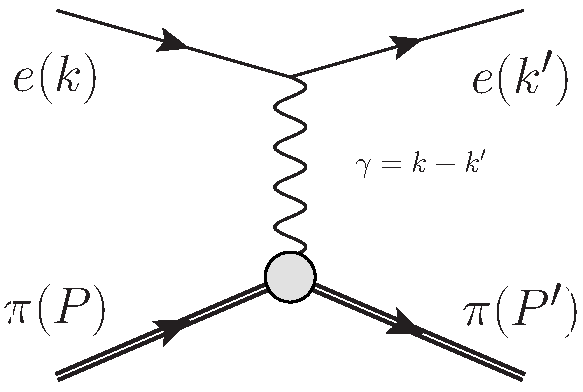
\includegraphics[width=0.55\textwidth]{figures/FF_gen} 
\caption{\footnotesize One-photon exchange pion elestic scattering. }\label{fig:FF_gen}
\end{center}
\end{figure}

The electron-hadron scattering experiments are well-proven technique since the electromagnetic part is well known. In this thesis we will focus on the pion as the target of scattering. The simplified picture of the corresponding experiment is given on Fig. \ref{fig:FF_gen}. The angular distributions of the cross section takes the form:
\beqa
	\frac{d\sigma}{d\Omega} =  \left( \frac{d\sigma}{d\Omega} \right)_{point-like} |F_\pi(q^2)|^2 \;,
	\label{pion:crosssection}
\eeqa
where $q=k-k^{\prime}$ is the momentum energy transferred between the electron and the pion. For the convenience purpose we consider the variable $Q^2 = - q^2$. The $F_\pi(q^2)$ is the pion electromagnetic form factor. For a static targets the form factor is given by Fourier transform of normalized charge distribution $\rho(\textbf{x})$:
\beqa
	F(\textbf{q}) = \int d^3x \rho(\textbf{x}) exp(i\textbf{q}\textbf{x})
	\label{pion:3d_FF}
\eeqa
If the momentum transfer is small we can expand the exponential in Eq. (\ref{pion:3d_FF}), obtaining:
\beqa
	F(\textbf{q}) = 1 - \frac{1}{6}\langle r^2 \rangle|\textbf{q}^2| + ...
\eeqa
As we see from the expansion the mean square radius of pion charge distribution is given by:
\beqa
\langle r^2 \rangle = - 6 \frac{dF(Q^2)}{dQ^2}
\eeqa
So the low momentum transfer electron-pion scattering measures only the mean square radius of the charge cloud of the pion. And this is expectable since the long wavelength virtual photon can only resolve the size of pion, but not its substructure. \\

According to Eq. (\ref{pion:crosssection}), the scattering on the pion as a spinless particle, in fully described by its form factor $F_\pi(Q^2)$. However we know that pion-photon vertex must be a Lorentz four-vector since photon is able to couple to it. This deduce the view of pion-photon vertex to the form:
\beqa
	(P^{\prime} + P)_\mu F_\pi(Q^2)
	\label{pion:FF_vertex}
\eeqa
From another side the pion-photon vertex can be written in a general form as:
\beqa
	\left\langle \pi(P^{\prime}) |J_\mu | \pi(P) \right\rangle\;,
	\label{pion:current_vertex}
\eeqa
where $\left\langle \pi(P) |\right. $ is the wave function of incoming pion, $\left. | \pi(P) \right\rangle $ is the wave function of outgoing pion and $J_\mu$ is pion's electromagnetic current. Obviously the Eq. (\ref{pion:FF_vertex}) is equal to Eq. (\ref{pion:current_vertex}), thus providing the route to calculate pion form factor:
\beqa
	\left\langle \pi(P^{\prime}) |J_\mu | \pi(P) \right\rangle = (P^{\prime} + P)_\mu F_\pi(Q^2)
	\label{pion:FF_relation}
\eeqa
So in order to obtain the electromagnetic pion form factor $F_\pi(Q^2)$ we need to know pion wave-function $\left. | \pi(P) \right\rangle$, which explicit view was established in Chapter \ref{chap:BSE} and is given by:
\beqa
	\left. | \pi(P) \right\rangle = \chi(k;P) = S(k + P/2)\Gamma(k;P)S(k - P/2)
\eeqa
and pion's electromagnetic current $J_\mu$. The current can be obtained by "gauging" the quark-quark scattering kernel $K$. \\

A description of systematic approach how to couple external gauge field was given by \cite{Sanchis-Alepuz:2013iia}. Shortly, the evolution of two-body quark system is given by the amputated version of scattering matrix $T^{(2)}$. Thus the scattering matrix $T$ can be obtained by solving the following Dyson equation:
\begin{equation}
\displaystyle T=-iK-iKG_0T
\label{Gauging_1}
\end{equation}
where $G_0$ is the disconnected product of two full quark propagators and $-iK$ is the two-quark interaction kernel. When the two-quark system forms a bound state, the scattering matrix develops a pole at $P^2=-M^2$, and can be defined as:
\begin{equation}
\displaystyle T^{(2)}\approx \frac{\Gamma \bar \Gamma}{P^2+M^2}
\label{Gauging_2}
\end{equation}
Substituting \ref{Gauging_2} in \ref{Gauging_1} and keeping only the singular term, we arrive at the \BSE for two quark bound state:
\begin{equation}
\displaystyle \Gamma = -iKG_0\Gamma,\:\:\:\:\ or \:\:\:\: iK^{-1}\Gamma = G_0\Gamma, \:\:\:\: or \:\:\:\: i\bar{\Gamma}K^{-1}=\bar{\Gamma}G_0
\label{Gauging_3}
\end{equation}
Then a systematic procedure of coupling to external gauge field, introduced in \cite{Kvinikhidze:1998xn}, gives for $T^{(2)}$:
\begin{equation}
\displaystyle T^\mu = T(iK^{-1} K^\mu K^{-1} + G_0^\mu)T
\label{Gauging_4}
\end{equation}
The bound state electromagnetic current $J^\mu$ can be expressed at the pole by:
\begin{equation}
\displaystyle T^{(2), \mu} \approx \frac{\Gamma_f}{P^2_f+M^2_f}J^\mu\frac{\bar \Gamma_i}{P^2_i+M^2_i}
\label{Gauging_5}
\end{equation}
Substituting \ref{Gauging_5} in \ref{Gauging_4} and using \ref{Gauging_3} we get:
\begin{equation}
\displaystyle J^\mu= \Gamma_f (-iG_0 K^\mu G_0 + G_0^\mu) \Gamma_i
\label{pion:pion_EM_current}
\end{equation} 

In case of rainbow-ladder single-gluon exchange the interaction kernel involves only gluon, so the first term $K^{\mu}=0$ because gluon does not couple to photon directly. So only the second term in Eq. (\ref{pion:pion_EM_current}) contributes to the current and the pion form factor is given by following diagram:
\begin{figure}[h]
\centering
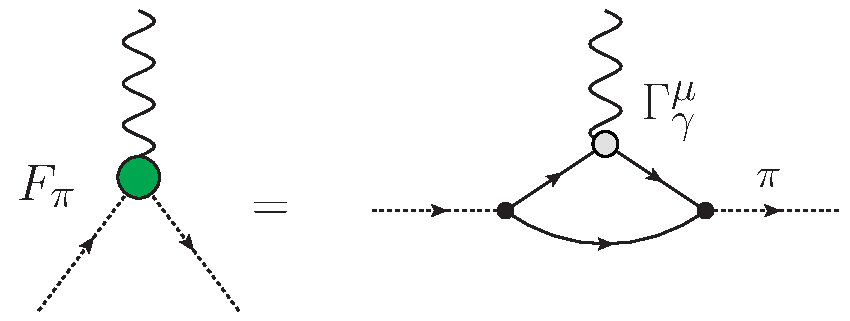
\includegraphics[width=0.7\textwidth]{figures/FF_RL}
\caption{\label{fig:FF_RL}\footnotesize Diagrams that contribute to pion form factor in case of rainbow-ladder single gluon exchange. All internal vertexes and propagators are dressed.}
\end{figure} \\

In case of pion cloud effect included, the gauging of the kernel is no longer zero $K^{\mu}\neq0$, since the kernel consists of quark-pion vertex and propagating pion and it is possible to couple a photon to the exchanging pion or to the quark-pion vertex. This fact generates two additional diagrams for the pion form factor. So they are given by diagrams in Fig. \ref{fig:FF_with_pi}. \\
\begin{figure}[h]
\centering
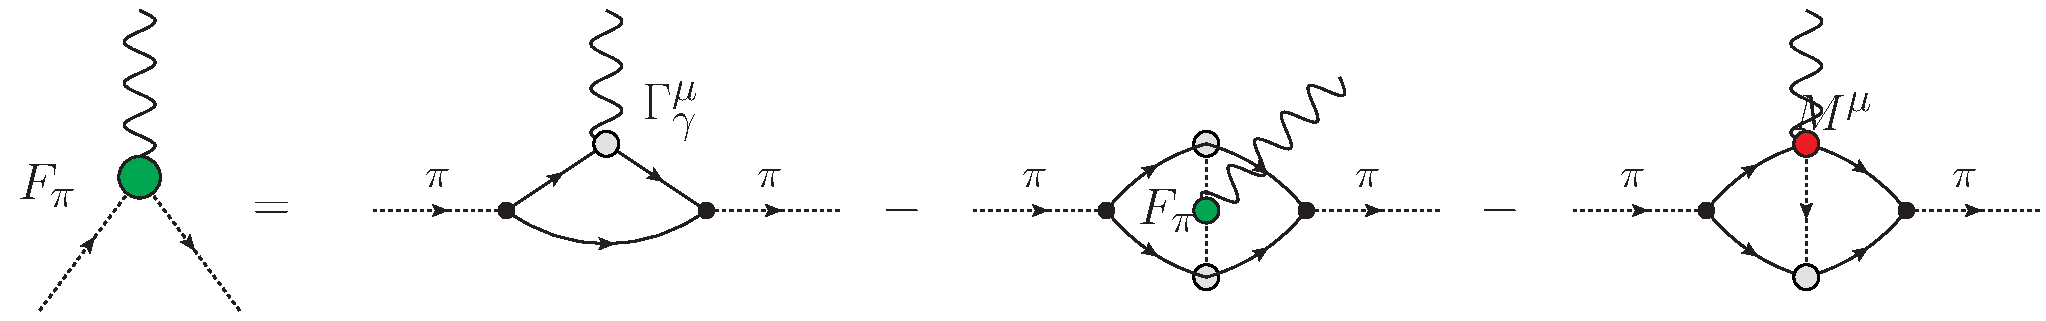
\includegraphics[width=0.99\textwidth]{figures/FF_with_pi}
\caption{\label{fig:FF_with_pi}\footnotesize Diagrams that contribute to pion form factor in case of pion cloud included. The second diagram (pion self-coupling) involves the pion form factor itself. The third diagram (seagull) involves the quark-pion-photon 4-vertex. All internal vertexes and propagators are dressed.}
\end{figure}
In comparison to rainbow-ladder the calculation become more complicated. The second diagram involves pion form factor in itself, so it requires to perform a self-consistent, iterative calculation, additionally complicated by two-loop integration. \\

Generally the pion-photon vertex depends on three momenta: $P_-$ - the initial momentum, $P_+$ - the final momentum and $Q$ - the momentum transferred. However, the momentum conservation $P_- + P_+ + Q = 0$ implies that only two momenta are independent. We choose the independent momenta to be the incoming photon momenta $Q$ and central-mass collision momentum $P$. The initial and final meson momenta can be written in terms of $Q$ and $P$ as $P_-=P-\frac{Q}{2}$ and $P_+=P + \frac{Q}{2}$, respectively. The condition of elastic scattering imposes additional constraints on $Q$ and $P$: $P_-^2=P_+^2=-m^2_{\pi}$,  $P^2=-\frac{Q^2}{4}-m^2_{\pi}$, so that only one remains independent. We use the specific momentum frame: 
\beqa
	Q_\mu &=& (0,0,Q,0)\\
	P_\mu &=& (0,0,0,P)\;,
\eeqa
where $Q$ and $P$ defined as:
\beqa
	Q &=& (Q^2)^{1/2}\\
	P &=& i\left( m^2_{\pi} + \frac{Q^2}{4}\right) ^{1/2}
\eeqa
After the frame is set we proceed to define the internal momenta routing for all diagrams in Fig. \ref{fig:FF_RL} and Fig. \ref{fig:FF_with_pi}.

\subsection*{Diagram A: Rainbow-ladder}
The first diagram A is given on Fig. \ref{fig:FF_A}.
\begin{figure}[h]
\centering
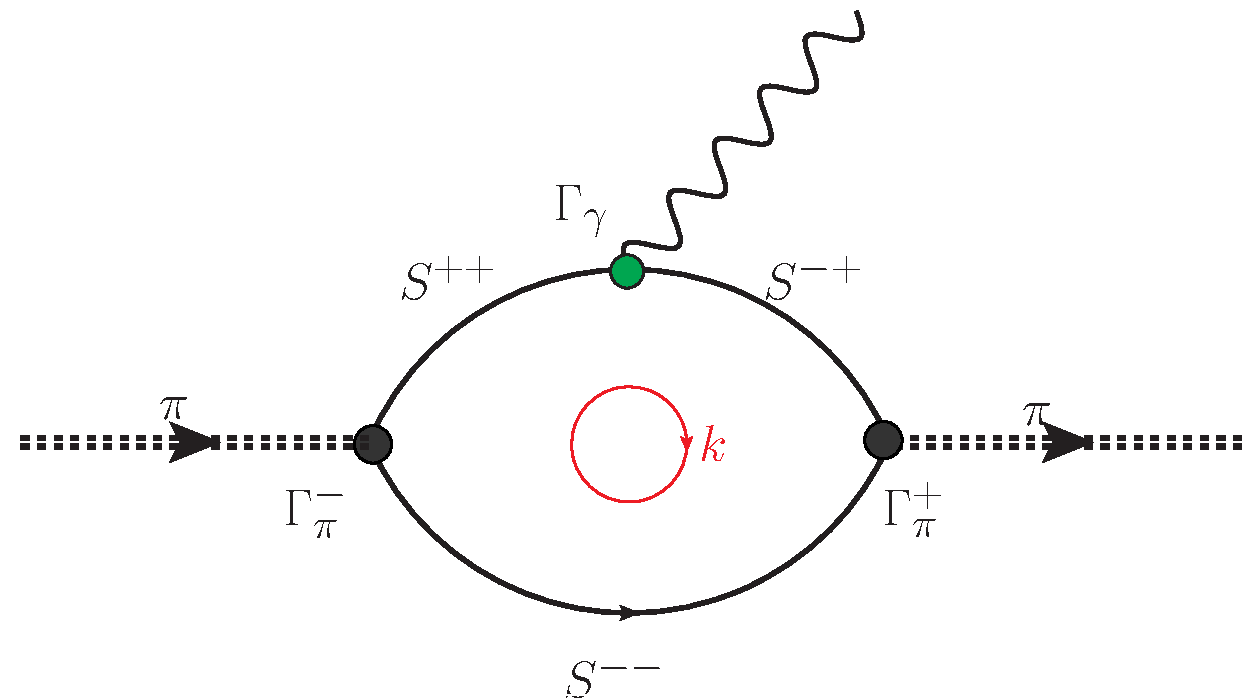
\includegraphics[width=0.7\textwidth]{figures/FF_A}
\caption{\label{fig:FF_A}\footnotesize The first diagram, common for the rainbow-ladder single gluon exchange and pion cloud effect. All internal vertexes and propagators are dressed.}
\end{figure}
According to the momenta routing choice the dressed vertexes and propagators have to evaluated on the following momenta:
\beqa
	\Gamma_{\pi}^-(k+Q/4,P_-)\;, & S^{++}(k + Q/2 + P/2) \\
	\Gamma_{\pi}^+(k-Q/4,P_+)\;, & S^{-+}(k - Q/2 + P/2) \\
	\Gamma_{\gamma}(k-P/2,Q)\;, & S^{--}(k - Q/2 - P/2)
\eeqa
where $k$ is integration momentum. The explicit notation of the corresponding to diagram A integral is following:
\beqa
	\frac{P_{\mu}}{P^2} \int \frac{d^4k}{(2\pi)^4} \Tr \left[ \Gamma_{\pi}^+ S^{-+} i\Gamma_{\gamma}^{\mu} S^{++} \Gamma_{\pi}^- S^{--} \right] 
\eeqa
Note that this notation is same in both cases - rainbow-ladder gluon exchange only or with pion cloud included.

\subsection*{Diagram B: Pion self-coupling}
The second diagram B illustrated on Fig. \ref{fig:FF_B}.
\begin{figure}[h]
\centering
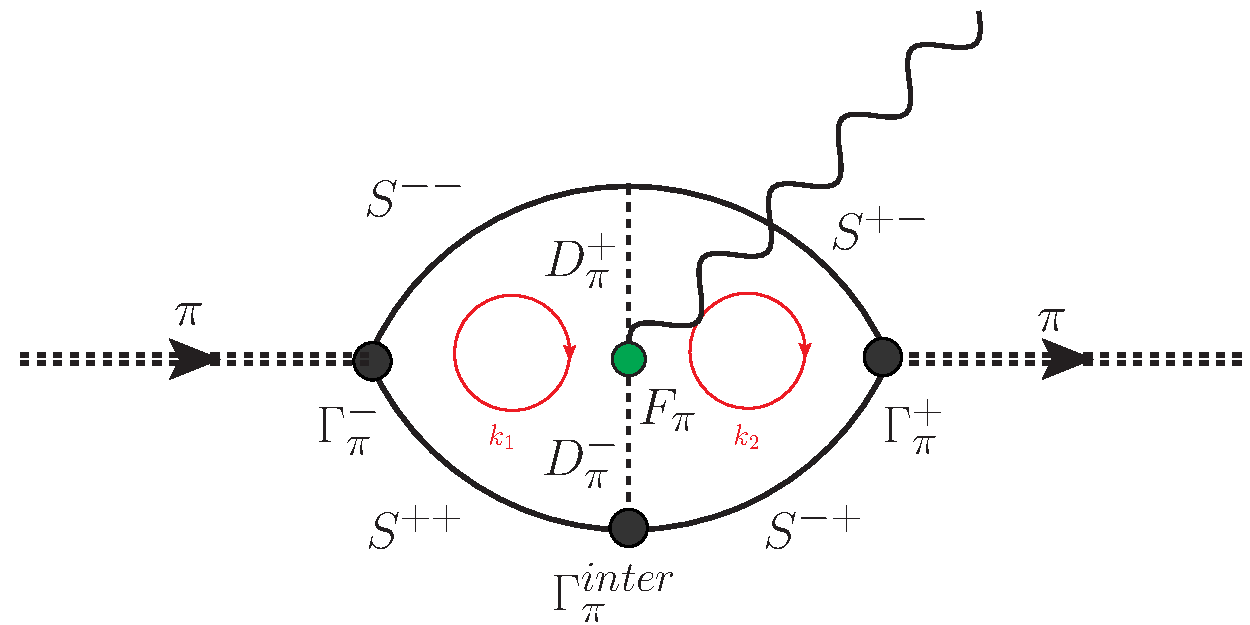
\includegraphics[width=0.7\textwidth]{figures/FF_B}
\caption{\label{fig:FF_B}\footnotesize The second diagram (pion self-coupling), which involves the pion form factor itself. All internal vertexes and propagators are dressed.}
\end{figure}
The momenta routing choice for the dressed vertexes and propagators reads as:
\beqa
	&\Gamma_{\pi}^-(k_1,P_-)\;, & S^{--}(k_1 - Q/4 - P/2)\\
	&\Gamma_{\pi}^+(k_2,P_-)\;, & S^{+-}(k_2 + Q/4 - P/2)\\
	&\Gamma_{\pi}^{inter}(\frac{k_1 + k_2 + P}{2})\;, & S^{-+}(k_2 - Q/4 + P/2)\\
	&F_\pi(Q^2)\;, & S^{++}(k_1 + Q/4 + P/2)\\
	&D_{\pi}^-(-Q/2 - k_1 + k_2)\;, & D_{\pi}^+(Q/2 - k_1 + k_2)
\eeqa
where $k_1$ and $k_2$ denotes integration momenta, flowing clock-wise as show by red contours on the diagram. $\Gamma_{\pi}^{inter}(\frac{k_1 + k_2 + P}{2})$ is the Bethe-Salpeter pion wave function, given in chiral approximation $\Gamma_{\pi}^{inter}(p) = \frac{B(p)}{f_{\pi}}$.

Denoting $S^{-+}\Gamma_{\pi}^{+}S^{+-} \equiv \chi_{\pi}^{+}$ and $S^{--}\Gamma_{\pi}^{-}S^{++} \equiv \chi_{\pi}^{-}$, the explicit view of the corresponding integral is following:
\begin{equation}
\begin{array}{c}
\displaystyle \frac{P_{\mu}}{P^2} \int\int \frac{d^4k_1}{(2\pi)}  \frac{d^4k_2}{(2\pi)} \Tr \left[  \chi_{\pi}^{+} \gamma_5 D_{\pi}^{+} (k_2 - k_1)_{\mu} F_{\pi} D_{\pi}^{+} \Gamma_{\pi}^{inter} \chi_{\pi}^{-} \right] 
\end{array}
\label{Diagram_B}
\end{equation} 
where $D_{\pi}^{\pm} = \frac{1}{\pm\frac{Q}{2} - k_1 + k_2 + m_{\pi}^2}$ are pion propagators. \\

It can be checked numerically that this diagram is zero, since the it is the internal loop integration momenta $k_1, k_2$ are equivalent. Hence we can split the Eq. \ref{Diagram_B} into the difference of the two double loop integrals and then in one of them perform a momenta permutation $k_1 \leftrightarrow k_2$ due to their symmetry. This would give us the same integral as the first and therefore their difference is zero.

\subsection*{Diagram C: Seagull}
The third diagram C displayed on Fig. \ref{fig:FF_C}. 
\begin{figure}[h]
\centering
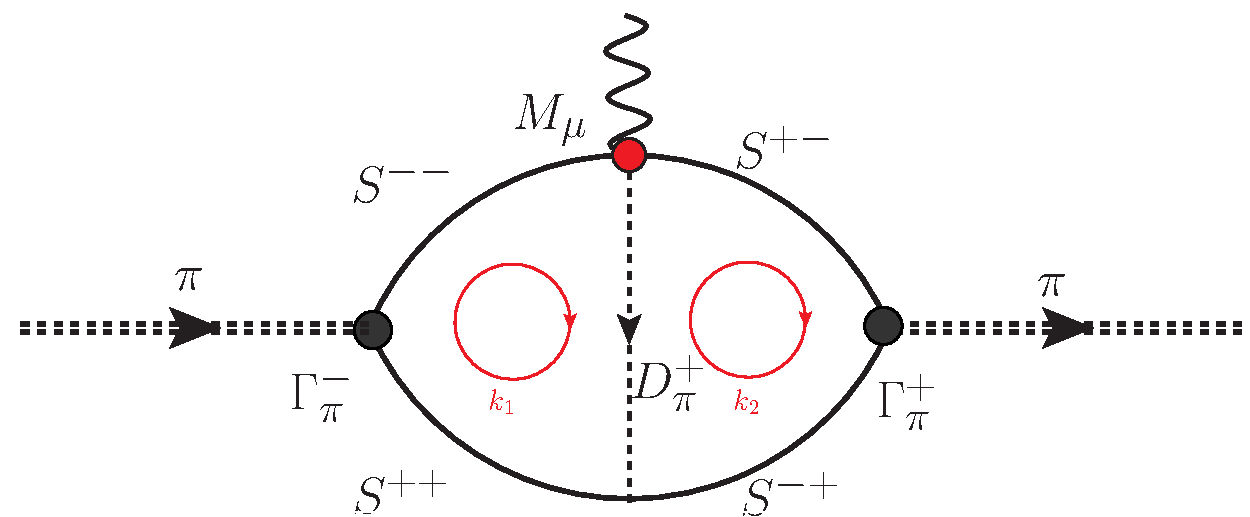
\includegraphics[width=0.7\textwidth]{figures/FF_C}
\caption{\label{fig:FF_C}\footnotesize The third diagram (seagull), which involves the \textit{ansatz} for the quark-pion-photon 4-vertex. All internal vertexes and propagators are dressed.}
\end{figure}
The momenta routing is similar to second diagram and set as following:
\beqa
	&\Gamma_{\pi}^-(k_1,P_-)\;, & S^{--}(k_1 - Q/4 - P/2)\\
	&\Gamma_{\pi}^+(k_2,P_-)\;, & S^{+-}(k_2 + Q/4 - P/2)\\
	&M_{\mu}(\frac{k_1 + k_2 - P}{2})\;, & S^{-+}(k_2 - Q/4 + P/2)\\
	&D_{\pi}^+(Q/2 - k_1 + k_2)\;, & S^{++}(k_1 + Q/4 + P/2)
\eeqa
As well as in previous diagram, $k_1$ and $k_2$ denotes integration momenta, flowing clock-wise as show by red contours on the diagram. $M_{\mu}$ is the \textit{ansatz} for the quark-pion-photon 4-vertex, derived in \cite{s100500070078} and it reads as:
\begin{equation}
\begin{array}{c}
\displaystyle M_\mu(q)=e_q\frac{(4q-Q)_\mu}{4q \cdot Q-Q^2} \left( \chi(q-Q/2) - \chi(q) \right) 
\displaystyle + e_q\frac{(4q+Q)_\mu}{4q \cdot Q+Q^2} \left( \chi(q+Q/2) - \chi(q) \right)
\end{array}
\label{Seagull_vertex}
\end{equation}
where $\chi(q) = S(q+P/2)\Gamma_{\pi}(q,P)S(q-P/2) |_{P^2=M^2}$ and $e_q$ is a quark charge, so the resulting integral reads as:
\begin{equation}
\begin{array}{c}
\displaystyle \frac{P_{\mu}}{P^2} \int\int \frac{d^4k_1}{(2\pi} \frac{d^4k_2}{(2\pi} \Tr \left[  \chi_{\pi}^{+} M_\mu(q) D_{\pi}^{+} \chi_{\pi}^{-} \right] 
\end{array}
\label{Diargam_C}
\end{equation} 
here as well as in previous diagram we denoting $S^{-+}\Gamma_{\pi}^{+}S^{+-} \equiv \chi_{\pi}^{+}$, $S^{--}\Gamma_{\pi}^{-}S^{++} \equiv \chi_{\pi}^{-}$ and $D_{\pi}^{+} = \frac{1}{\frac{Q}{2} - k_1 + k_2 + m_{\pi}^2}$ is pion propagator. Note that there is of course similar diagram, just  mirrored and therefore the quark-pion-photon 4-vertex is $M_{\mu}(\frac{k_1 + k_2 + P}{2})$ and pion propagator is $D_{\pi}^{-} = \frac{1}{-\frac{Q}{2} - k_1 + k_2 + m_{\pi}^2}$.\\

\subsection*{Pion Form Factor}
As we saw in the DSE/BSE approach, pion cloud effects enter in the dynamical properties as a form factor in various ways: starting from solving the quark DSE the pion exchange contributes to dressed quark propagator; through the appropriate two-body kernel the pion cloud impacts on Bethe-Salpeter amplitudes of pion and photon; and finally after kernel gauging procedure the pion cloud exposes itself by producing extra diagrams for the calculation of form factor. 
\begin{figure}[!]
\centering
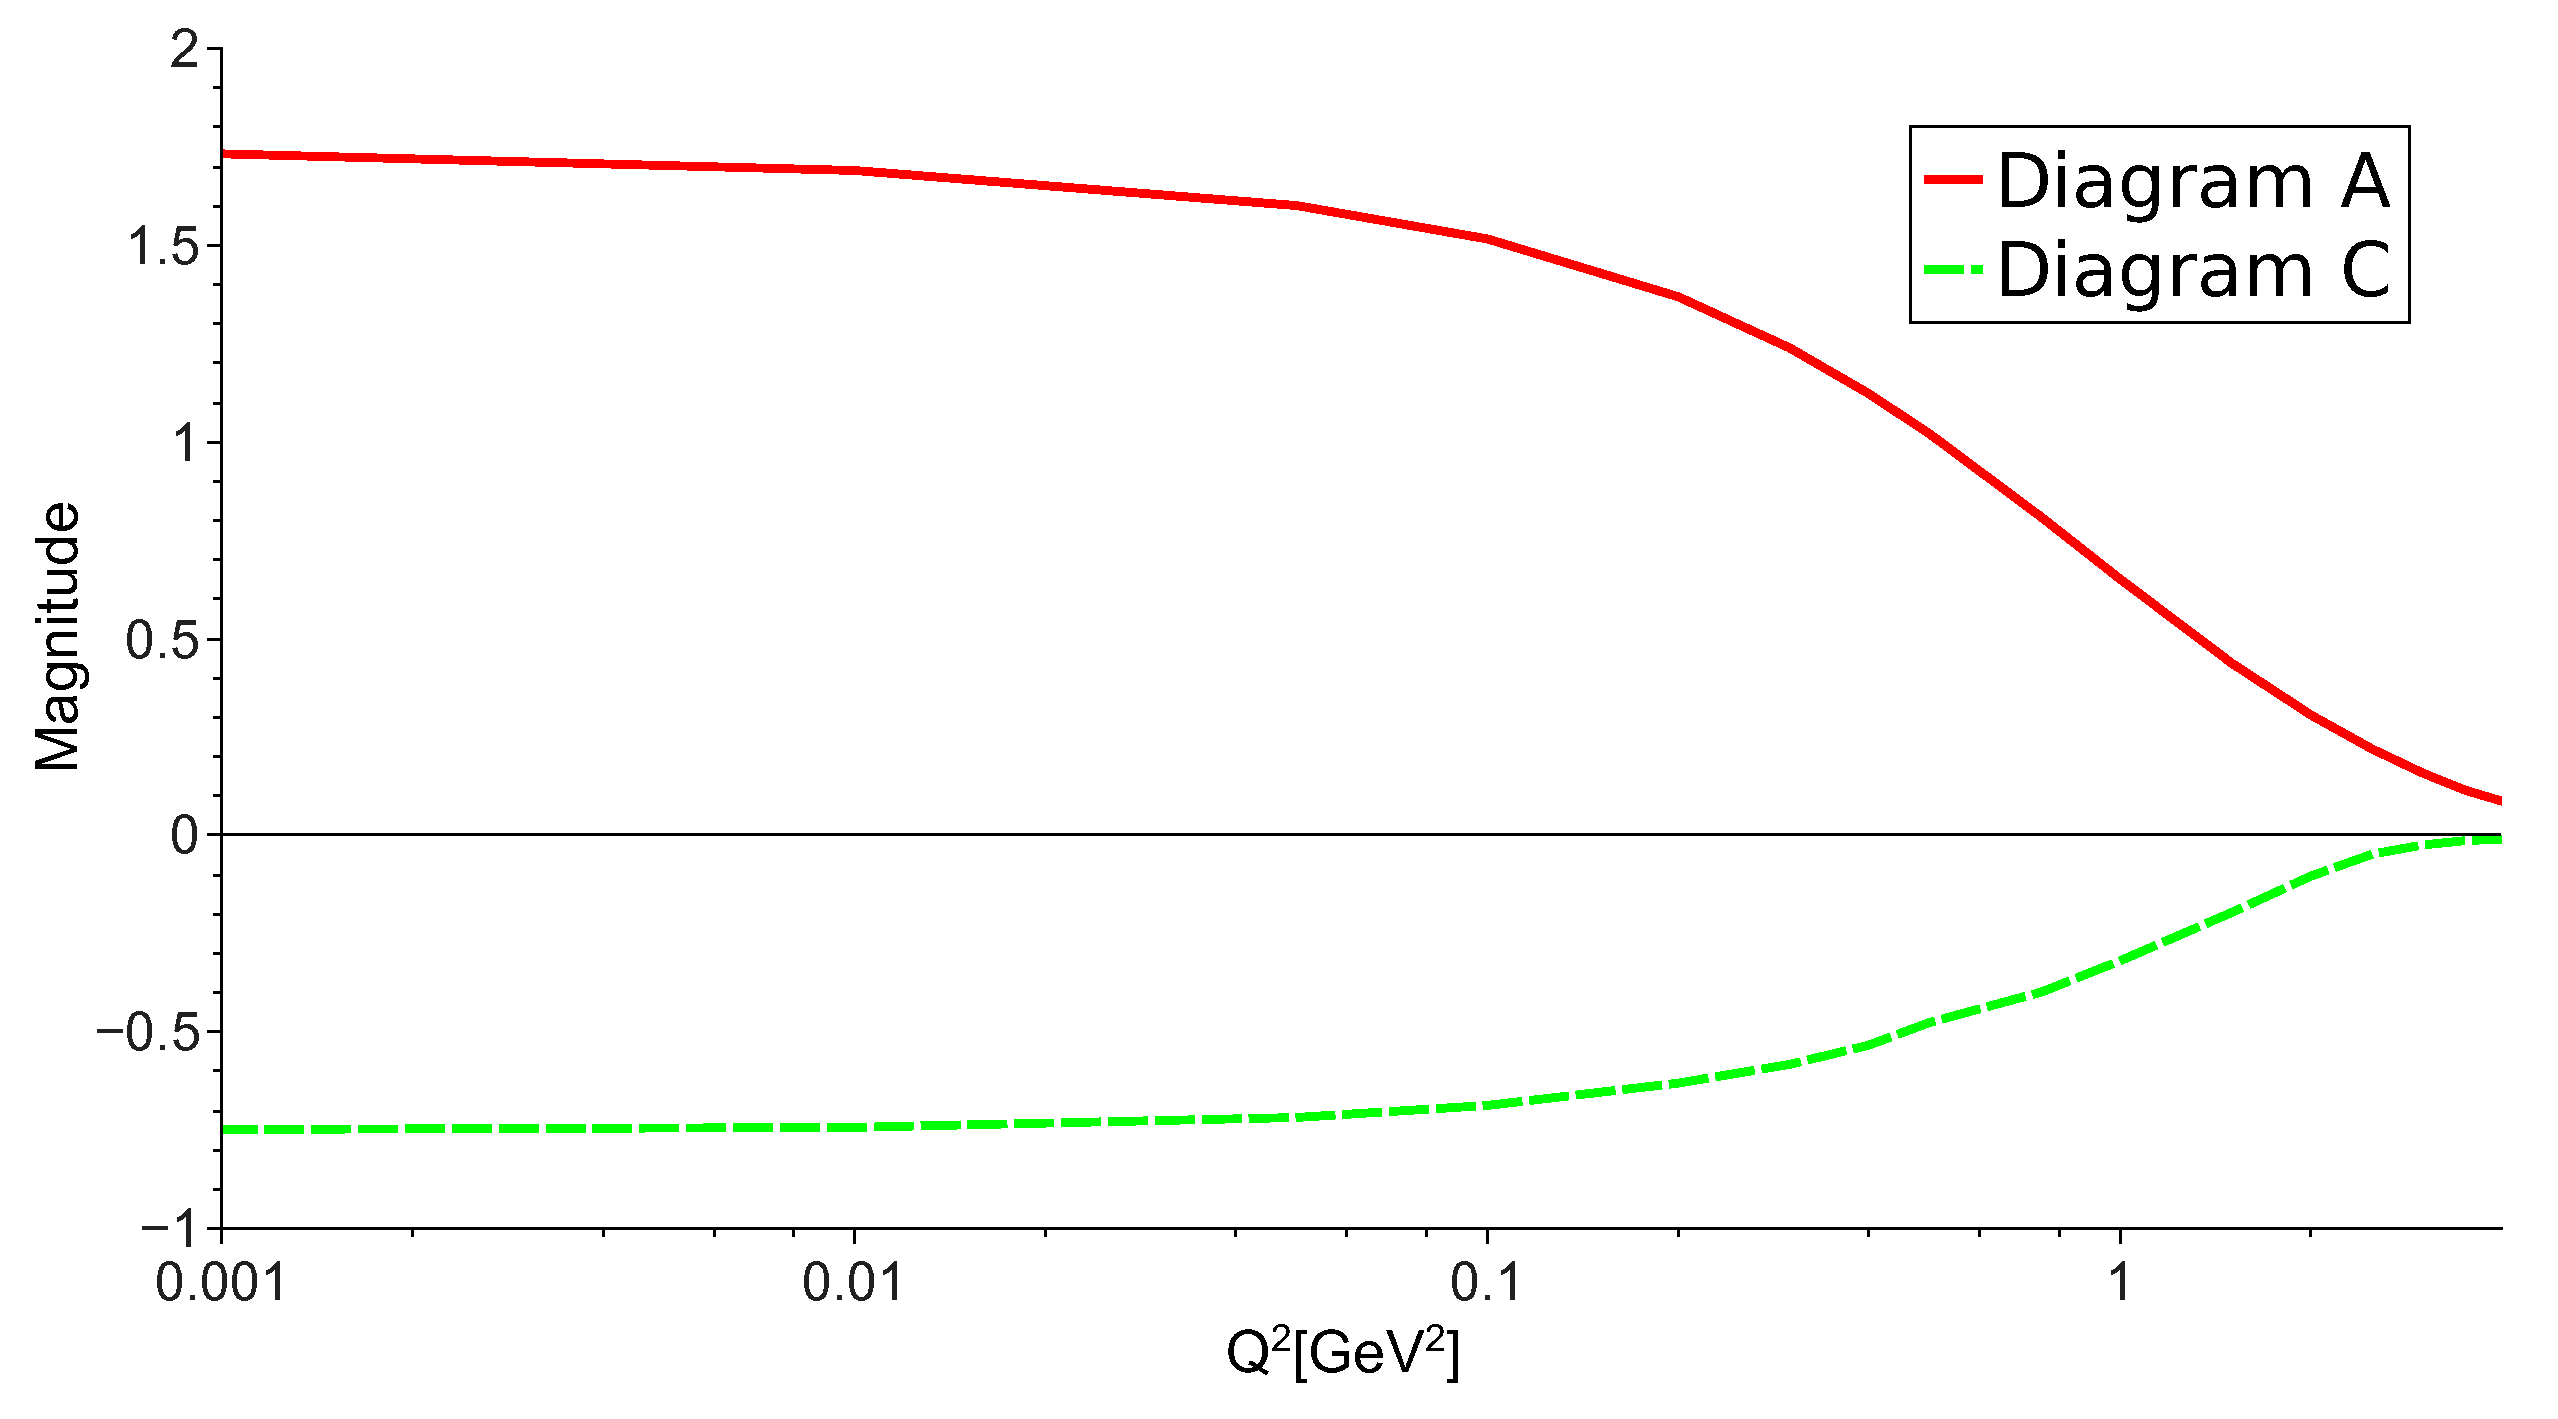
\includegraphics[width=0.99\textwidth]{figures/FF_A_C}
\caption{\label{fig:FF_A_C}\footnotesize The contribution of A and C diagrams for comparison as a function of $Q^2$. Sum of them at $Q^2=0$ equal $F_\pi(Q^2=0) = 1$ fulfilling the Ward-Takahashi identity and conserving the electric charge. The gluon parameters are $\Lambda=0.84$ and $\eta=1.8$.}
\end{figure} \\

Since as it was mentioned the pion cloud piece enters into the calculation recipe on various levels it is crucial to keep under control by tracking the Ward-Takahashi identity and charge conservation. On the form factor level this implies $F_\pi(Q^2=0)=1$. This fact can be easily understood from the qualitative point of view: if we probe the charged pion by very long wave-length photon we will not resolve any internal structure, the point-like charged pion. If the resulting form factor at $Q^2=0$ is $F_\pi(Q^2=0)=1$, then this signal us that the normalization of the BSA was done
correctly and the electric charge is conserved. In case of rainbow-ladder gluon this would require us to calculate only one diagram given on Fig. \ref{fig:FF_RL}, however in case of pion cloud effect all three diagrams on Fig. \ref{fig:FF_with_pi}. Fortunately the second diagram B is zero everywhere on $Q^2$ due to momenta routing specificness, and therefore does not contribute to the form factor. This fact leaves us with two diagrams: A and C, they contribution to pion form factor is shown on Fig. \ref{fig:FF_A_C}.
\begin{figure}[h]
\centering
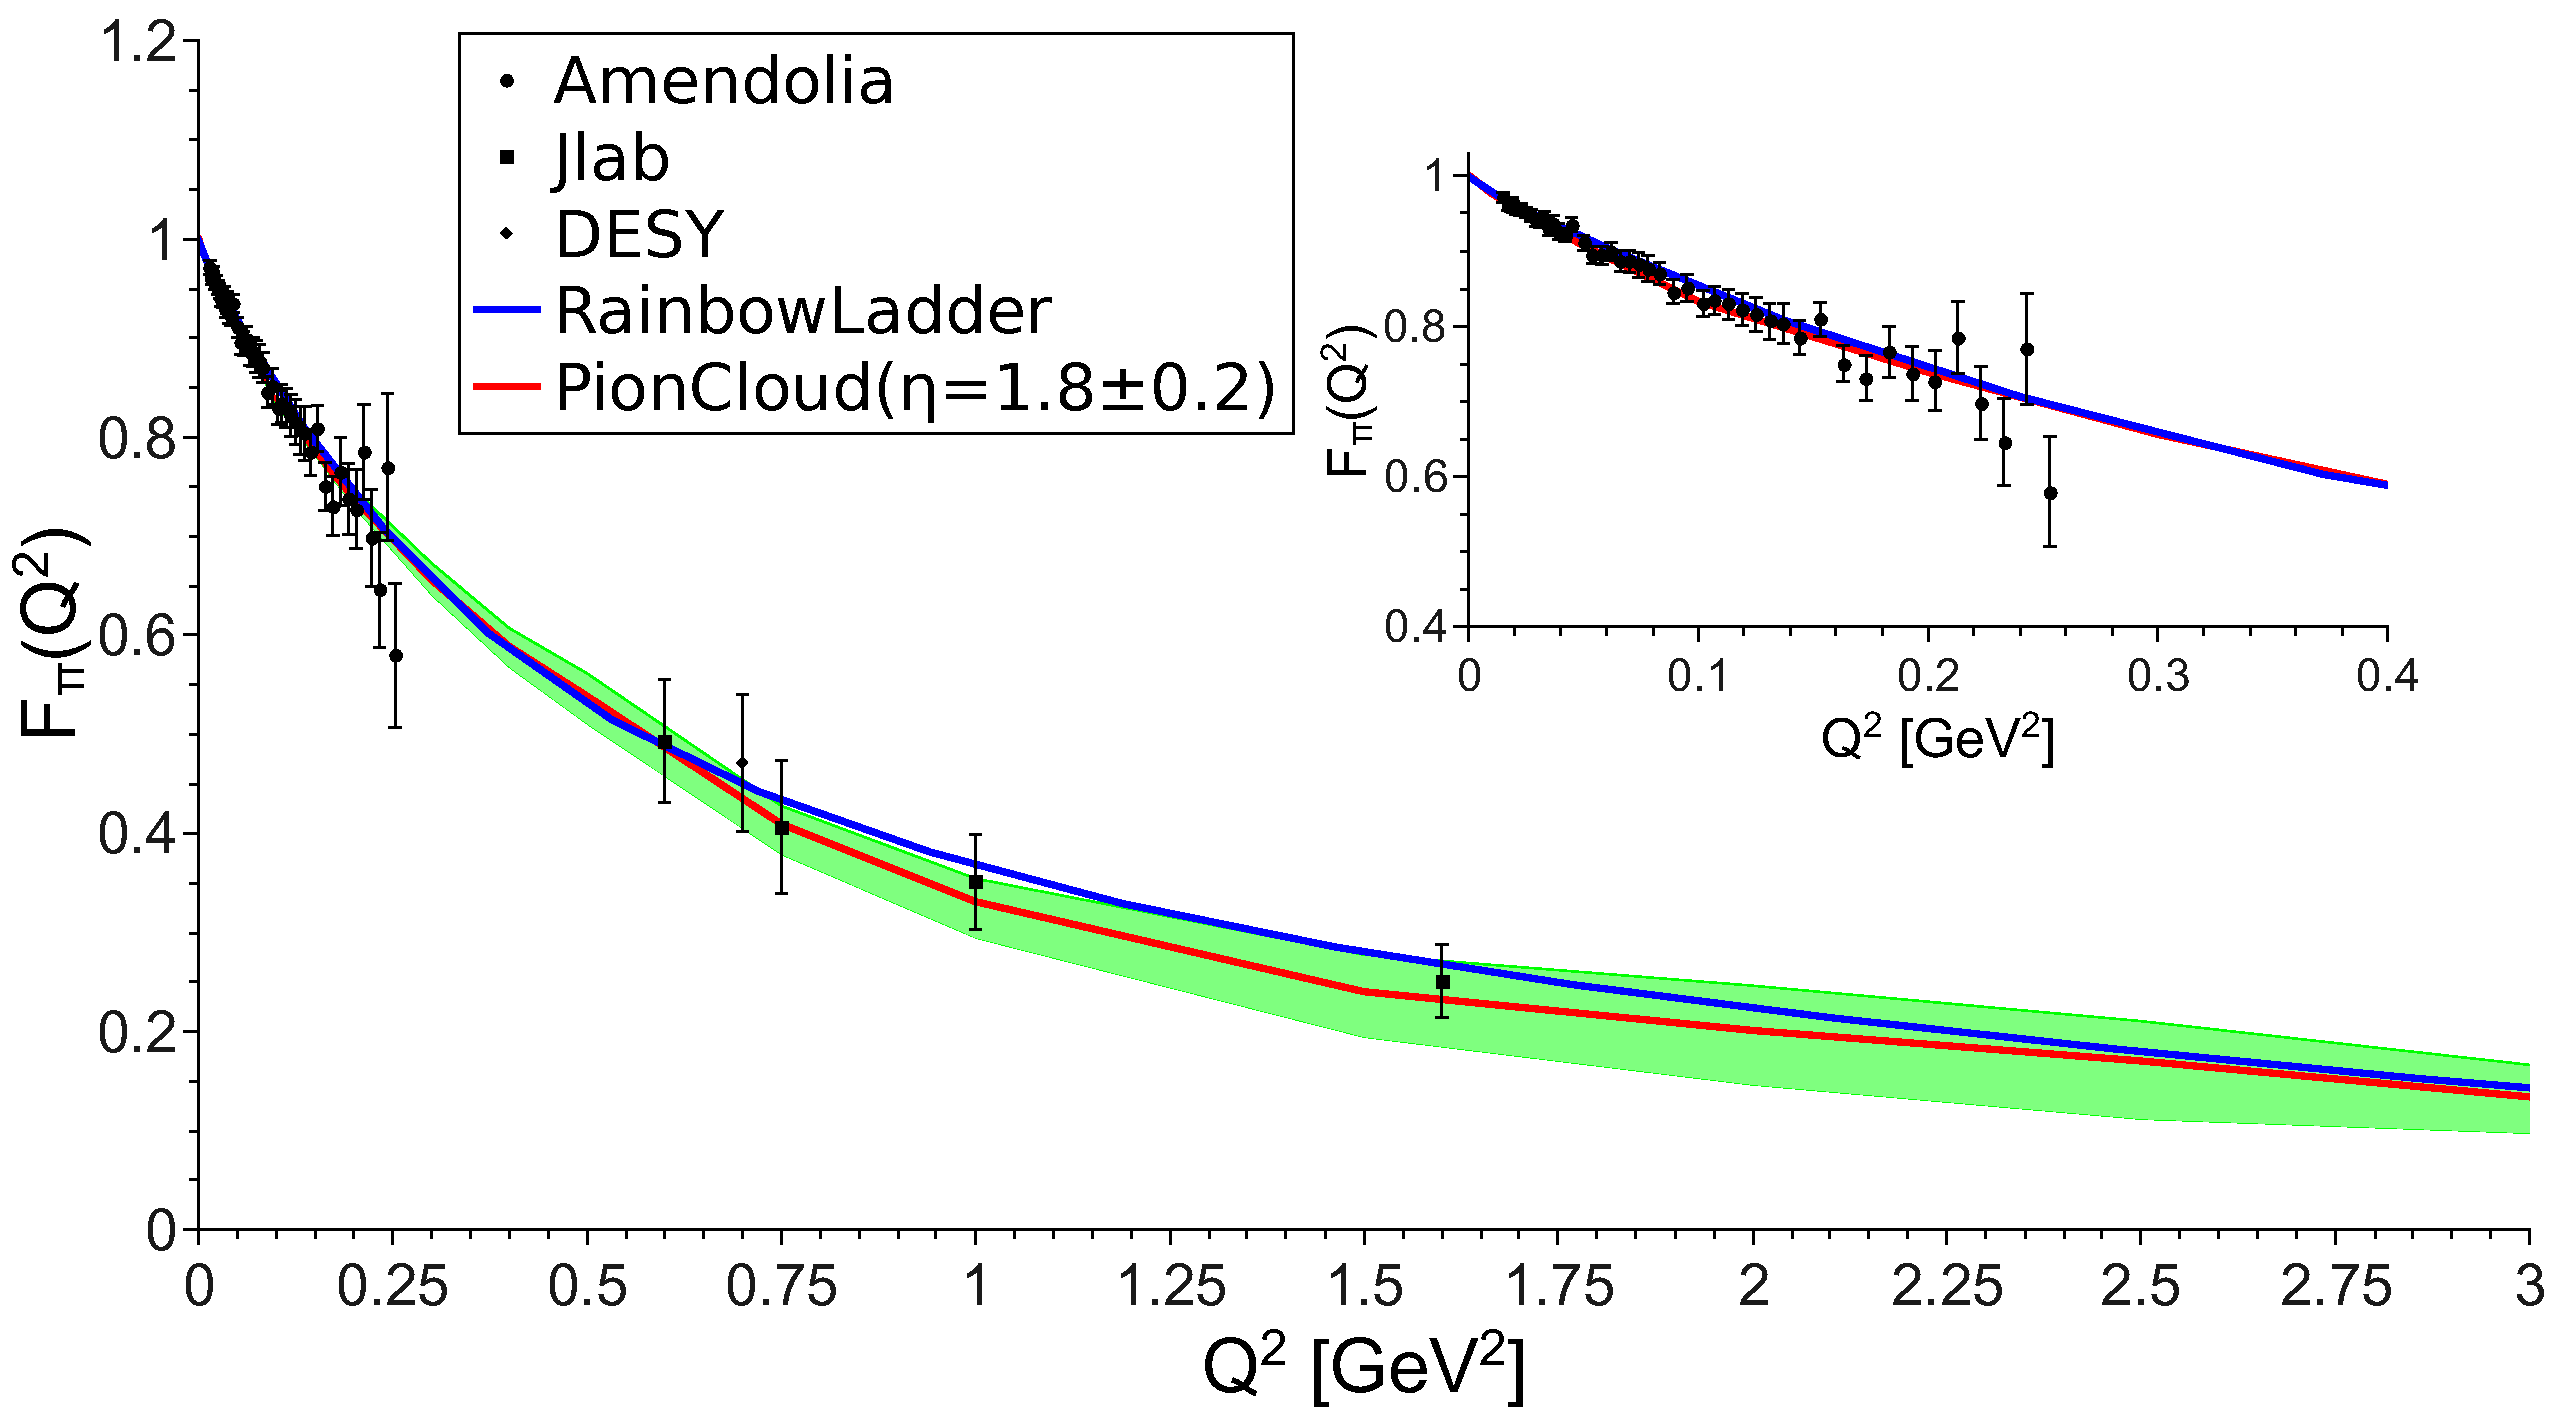
\includegraphics[width=0.99\textwidth]{figures/FF_RL_PS}
\caption{\label{fig:FF_RL_PS}\footnotesize The resulting pion form factor for two types of kernels: blue lines correspond to single rainbow-ladder gluon exchange only; red line to the gluon exchange with pion cloud effect. The green area correspond to $\eta$ parameter variation. The experemental data obtained from \cite{Amendolia:1986wj,Volmer:2000ek}.}
\end{figure} \\

In Fig. \ref{fig:FF_RL_PS} we present numerical results for the pion form factor carried out within two schemes: rainbow-ladder single gluon exchange and pion cloud effect impact. We compare them to available experimental data, obtained within \cite{Amendolia:1986wj,Volmer:2000ek}. Firstly we observe that both of truncations provide the charge conservation and fulfil the Ward-Takahashi identity as the calculated form factor fulfils the condition $F_\pi(Q^2=0)=1$. The interesting discrepancy arises at the intermediate range of $Q^2$. For $0.75\; \text{GeV}^2 < Q^2 < 1.75\; \text{GeV}^2$ the pion form factor with pion cloud deviates from rainbow-ladder result at the level of 10 percents. The qualitative explanation is the following: at very low $Q^2$ photon resolves the pion as a whole thing without any substructure, whether at very large $Q^2$ it resolves the separate quarks and at aforementioned intermediate range of $Q^2$ the photon "sees" the pion quark core and the pion cloud surrounding it. Obviously this does not happen in case if the only gluon exchange taken into account. The observation that the form factor with pion cloud is smaller than rainbow-ladder one reflects the fact that the virtual pions provide the charge screening effect in that kinematic range. Unfortunately, the experimental data in that region does not allow to distinguish between the single gluon exchange and the pion cloud picture due to big error bars. However it is potentially plausible to estimate the pion cloud effect with improved experimental statistics. At the ultraviolet limit both curves tend to merge since the pion cloud effect diagram C fades faster with growing $Q^2$ that diagram A, according to Fig. \ref{fig:FF_A_C}, because of the specifics of momenta routing.




